\section{Error Mitigation Patterns}


Die Error Mitigation Patterns versuchen, den Fehler an Ort und Stelle, an der er aufgetreten ist, zu behandeln und schliessend das System von diesem Punkt aus weiter arbeiten zu lassen. Dies steht im Gegensatz zu den Vorhergehenden Error Recovery Patterns, welche das System durch Springen in einen fehlerfreien Zustand wieder zur normalen Ausführung bringen.

Viele Fehler, die abgeschwächt (mitigated) werden können, betreffen die Zeit oder Ressource (zu wenig CPU-Zeit, zu viele Requests, zu wenig Ressourcen).

\begin{figure}[H]
	\centering
	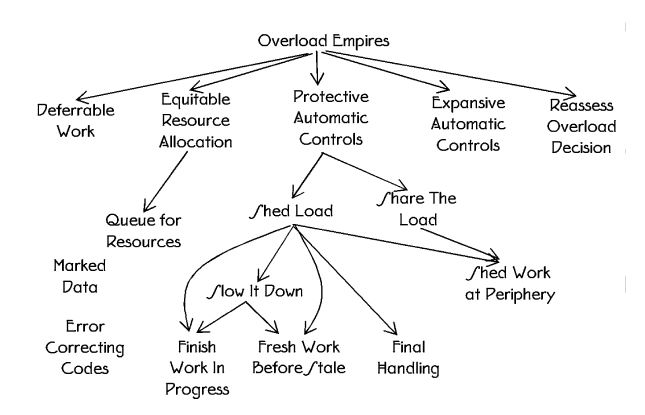
\includegraphics[width=\textwidth]{content/faulttolerance/images/MitigationPatterns_Dependecy.JPG}
	\caption{MitigationPatterns Dependecy}
\end{figure}


\begin{figure}[H]
	\centering
	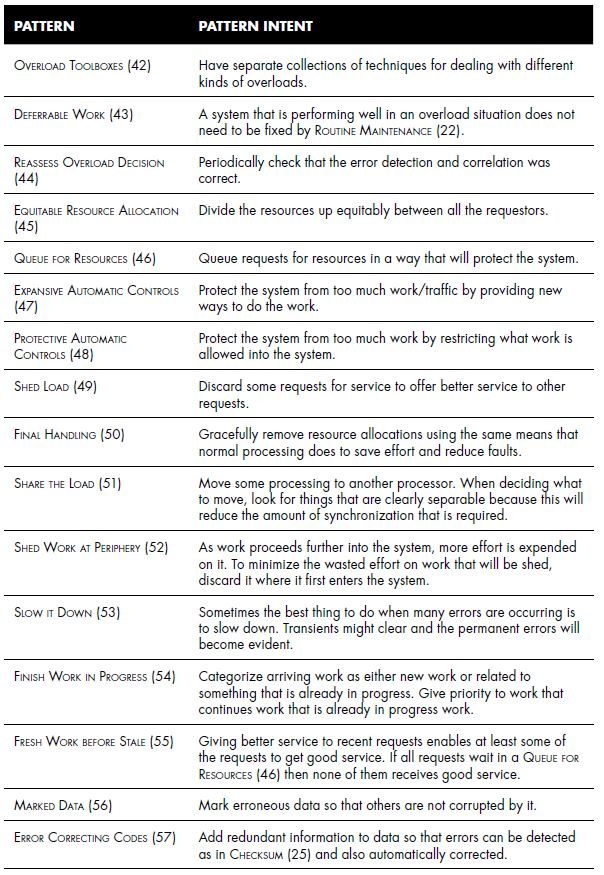
\includegraphics[width=\textwidth]{content/faulttolerance/images/MitigationPatterns.JPG}
	\caption{MitigationPatterns}
\end{figure}



